\newpage
\section{Layout design for MOS transistor}

\subsection{NMOS}
\itemmini{Design the layout for an NMOS\_VTL (120n/60n), ensuring compliance with Design Rule Check (DRC). Verify the corresponding throught Layout Versus Schematic (LVS) confirmation.}\\ 

\itemmini{Schematic}\\

\begin{figure}[H]
	\centering
	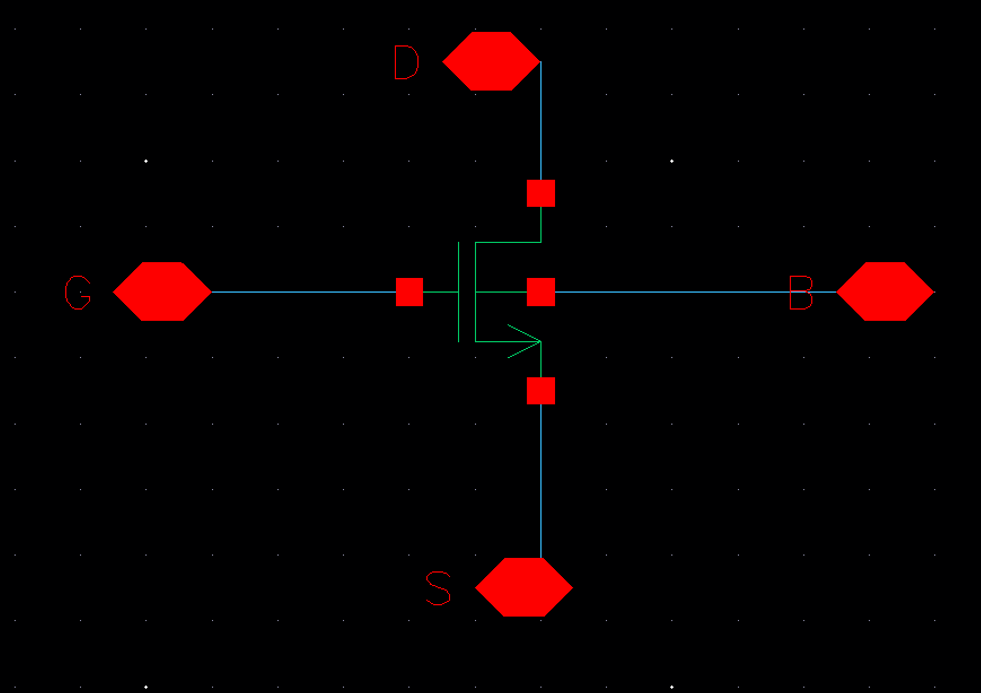
\includegraphics[width=.7\linewidth]{sections/pic/EX4_NMOS_schematic.png}
	\caption{Schematric NMOS ($(W/L) = (120n/90n)$).}
	\label{f_EX4_NMOS_schematic}
\end{figure}

\itemmini{Layout}\\

\begin{enumerate}[leftmargin=*, label = Step \arabic*:]
	\item Add \textit{n-active} layer define the active region dimensions based on the schematic parameters.
	\item Add Poly layer following the Rule ($\text{Contact} \geq 65nm$ and $\text{Poly} \geq 50nm$).
%	\item Thêm lớp \textbf{pimplant|drw} và \textbf{nimplant|drw} phủ theo kích thước Active.
	\item  Create drain, source, and bulk connections.
	\item Draw \textit{p-well} ensure compliance with design rules
	\item Cover with Metal1 layer.
	\begin{figure}[H]
		\centering
		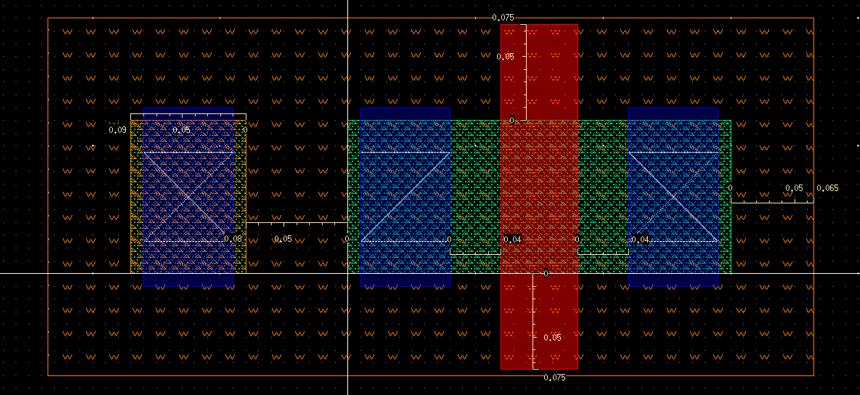
\includegraphics[width=.7\linewidth]{sections/pic/EX4_NMOS_metal.png}
		\label{f_EX4_NMOS_metal}
	\end{figure}
	\item Design the Gate structure includes: Contact, Metal1, and Poly.\\
	(\textit{Note: Gate Poly must adhere to distinct width/spacing rules (different from Active-to-Poly connections).}\\
	\begin{figure}[H]
		\centering
		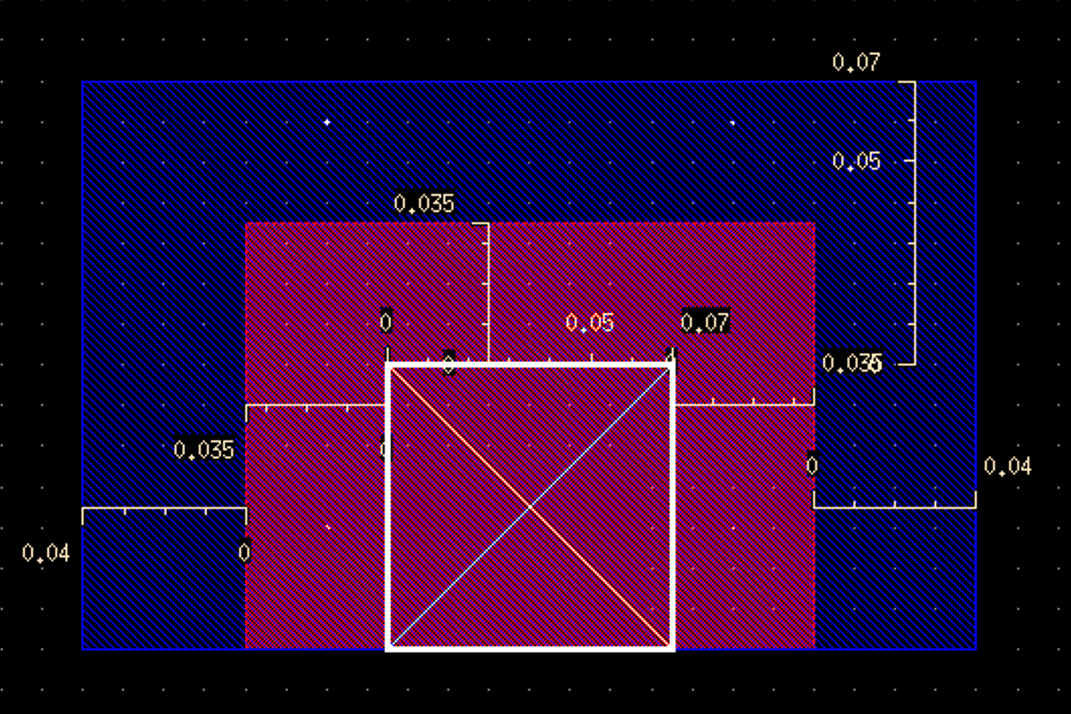
\includegraphics[width=.7\linewidth]{sections/pic/EX4_NMOS_gate.png}
		\label{f_EX4_NMOS_gate}		
	\end{figure}
	\item Add Metal2 and Vias.
	\begin{figure}[H]
		\centering
		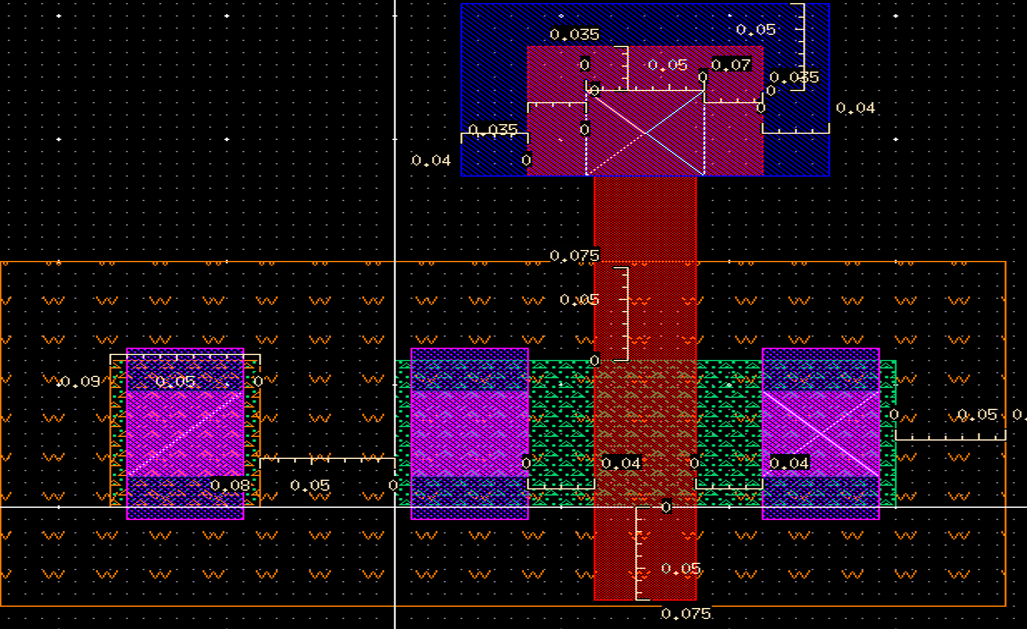
\includegraphics[width=.7\linewidth]{sections/pic/EX4_NMOS_metal2_vias.png}
		\label{f_EX4_NMOS_metal2_vias}
	\end{figure}
	\item Schematic-Layout Verification.
	\begin{figure}[H]
		\centering
		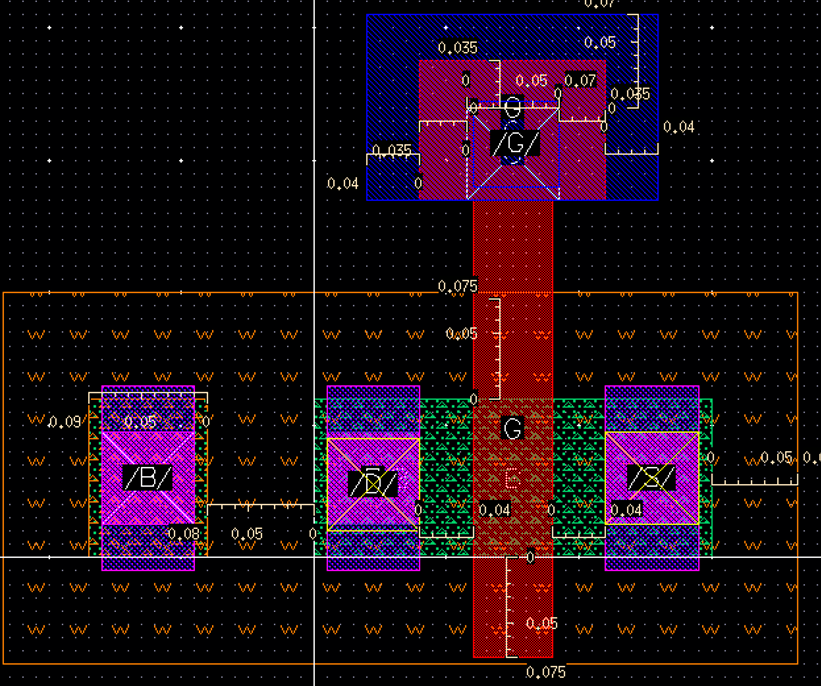
\includegraphics[width=.7\linewidth]{sections/pic/EX4_NMOS_layout_schematic.png}
		\label{f_EX4_NMOS_layout_schematic}
	\end{figure}
\end{enumerate}

\itemmini{Check DRC}\\

\begin{figure}[H]
	\centering
	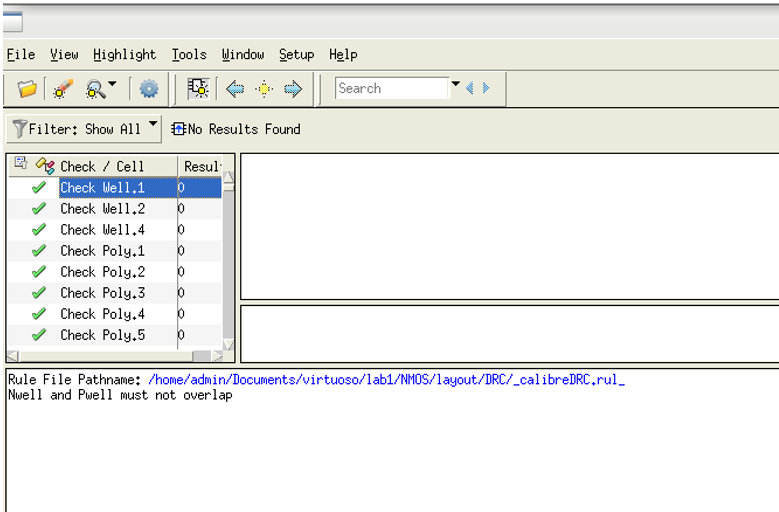
\includegraphics[width=.7\linewidth]{sections/pic/EX4_NMOS_DRC.png}
	\label{f_EX4_NMOS_DRC}
\end{figure}

\itemmini{Check LVS} \\

\begin{figure}[H]
	\centering
	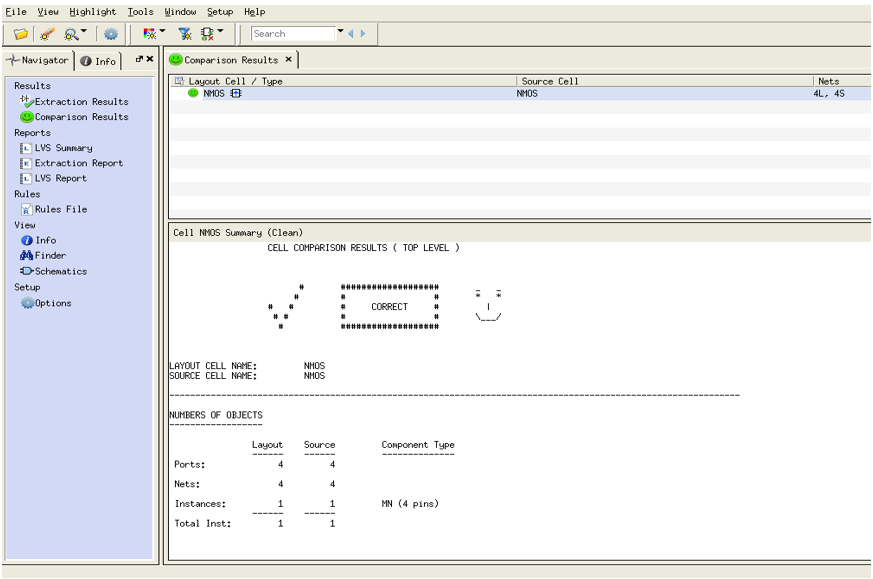
\includegraphics[width=.7\linewidth]{sections/pic/EX4_NMOS_LVS.png}
	\label{f_EX4_NMOS_LVS}
\end{figure}

\subsection{PMOS}
\itemmini{Design the layout for an PMOS\_VTL (50n/40n), ensuring compliance with Design Rule Check (DRC). Verify the corresponding throught Layout Versus Schematic (LVS) confirmation.}

\itemmini{Schematic}\\

\begin{figure}[H]
	\centering
	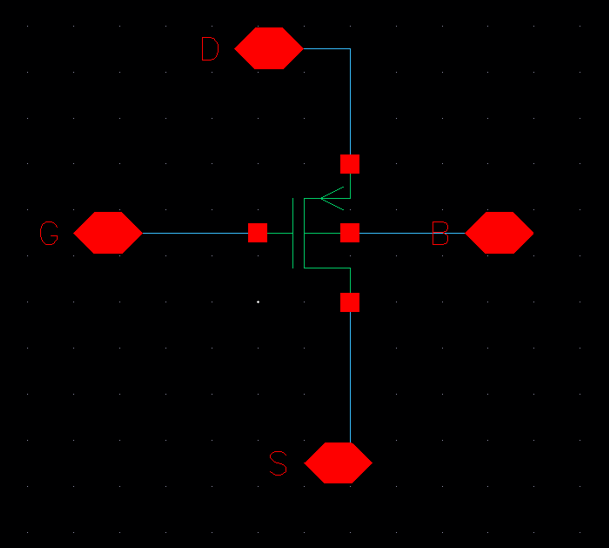
\includegraphics[width=.7\linewidth]{sections/pic/EX4_PMOS_schematic.png}
	\caption{Schematric PMOS ($(W/L) = (120n/90n)$).}
	\label{f_EX4_PMOS_schematic}
\end{figure}

\itemmini{Layout}\\

\begin{enumerate}[leftmargin=*, label = Step \arabic*:]
	\item Add \textit{n-active} layer define the active region dimensions based on the schematic parameters.
	\item Add Poly layer following the Rule ($\text{Contact} \geq 65nm$ and $\text{Poly} \geq 50nm$).
	%	\item Thêm lớp \textbf{pimplant|drw} và \textbf{nimplant|drw} phủ theo kích thước Active.
	\item  Create drain, source, and bulk connections.
	\item Draw \textit{p-well} ensure compliance with design rules
	\item Cover with Metal1 layer.
	\begin{figure}[H]
		\centering
		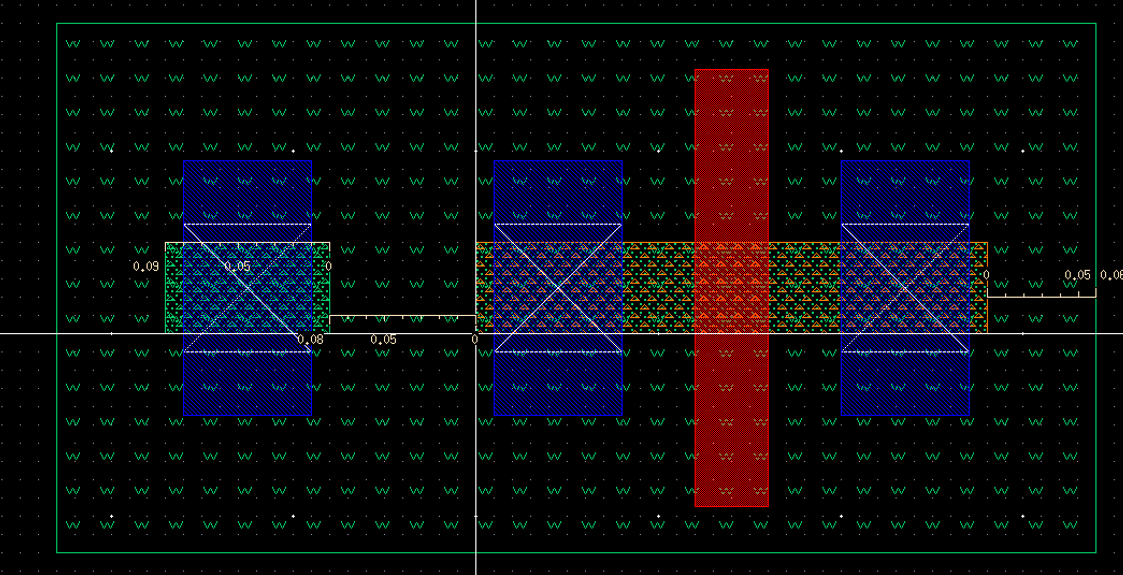
\includegraphics[width=.7\linewidth]{sections/pic/EX4_PMOS_metal.png}
		\label{f_EX4_PMOS_metal}
	\end{figure}
		\item Design the Gate structure includes: Contact, Metal1, and Poly.\\
	(\textit{Note: Gate Poly must adhere to distinct width/spacing rules (different from Active-to-Poly connections).}\\
	\begin{figure}[H]
		\centering
		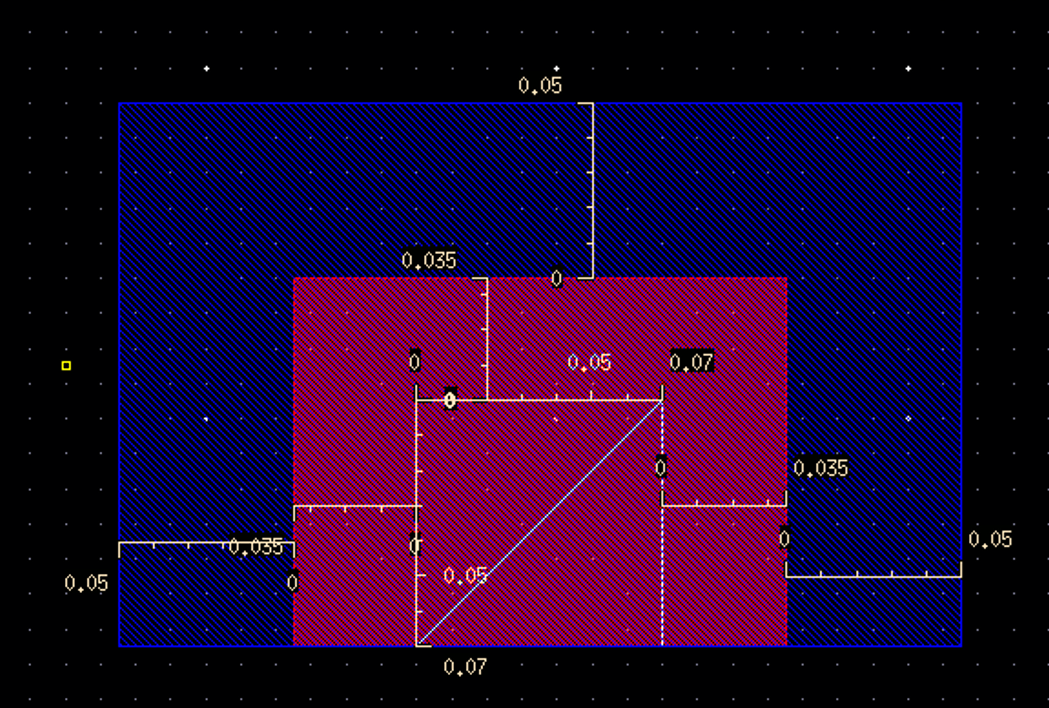
\includegraphics[width=.7\linewidth]{sections/pic/EX4_PMOS_gate.png}
		\label{f_EX4_PMOS_gate}		
	\end{figure}
	\item Add Metal2 and Vias.
	\begin{figure}[H]
		\centering
		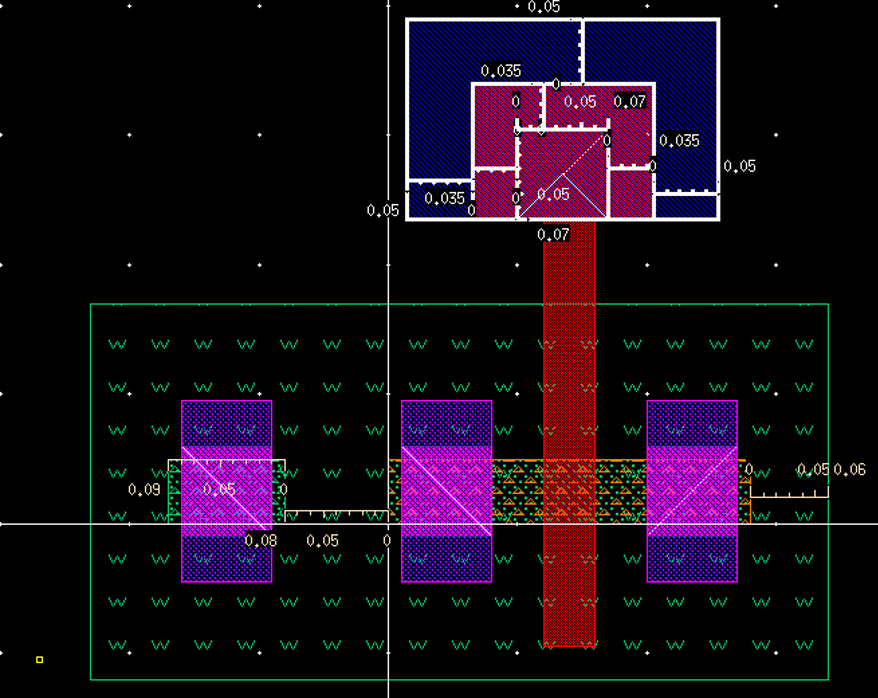
\includegraphics[width=.7\linewidth]{sections/pic/EX4_PMOS_metal2_vias.png}
		\label{f_EX4_PMOS_metal2_vias}
	\end{figure}
	\item Schematic-Layout Verification.
	\begin{figure}[H]
		\centering
		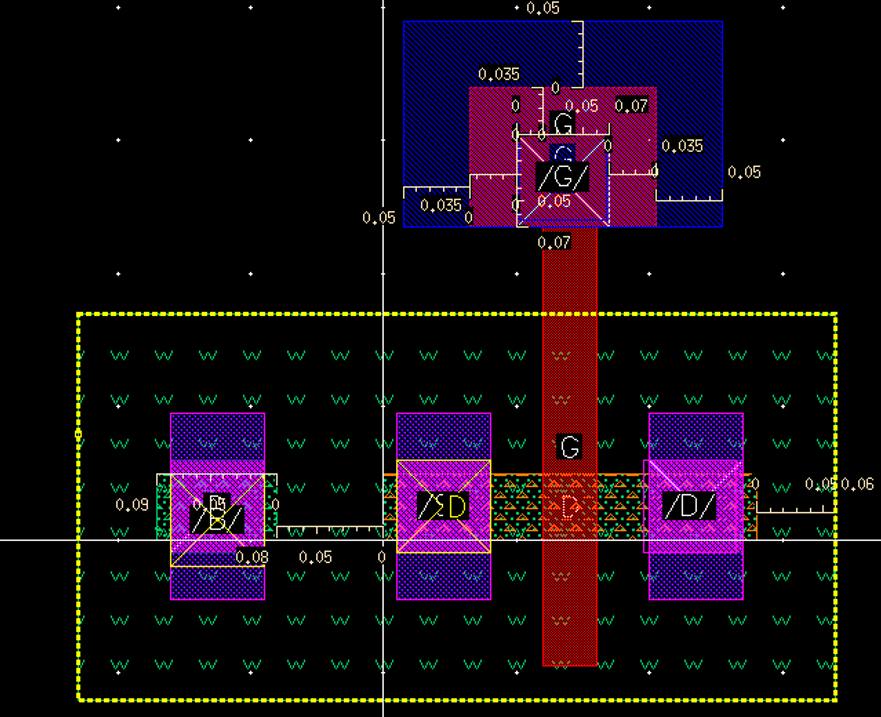
\includegraphics[width=.7\linewidth]{sections/pic/EX4_PMOS_layout_schematic.png}
		\label{f_EX4_PMOS_layout_schematic}
	\end{figure}
\end{enumerate}

\itemmini{Check DRC}\\

\begin{figure}[H]
	\centering
	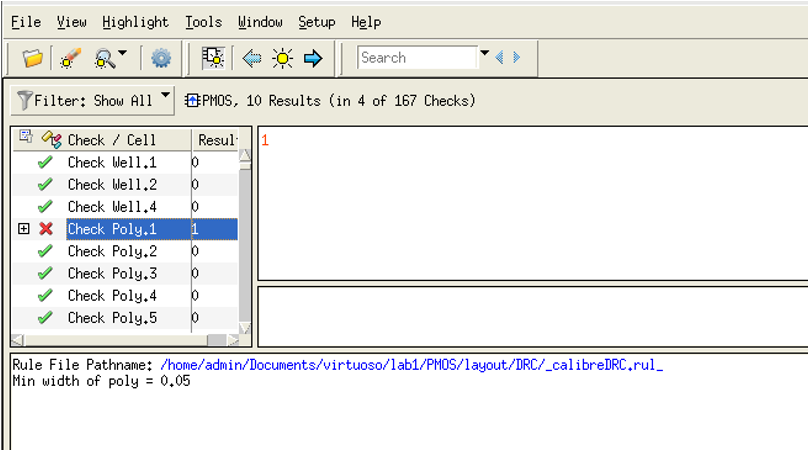
\includegraphics[width=.7\linewidth]{sections/pic/EX4_PMOS_DRC.png}
	\label{f_EX4_PMOS_DRC}
\end{figure}

The error is due to Poly requiring a minimum of $50n$ but the requirement is set at $40n$.

\begin{figure}[H]
	\centering
	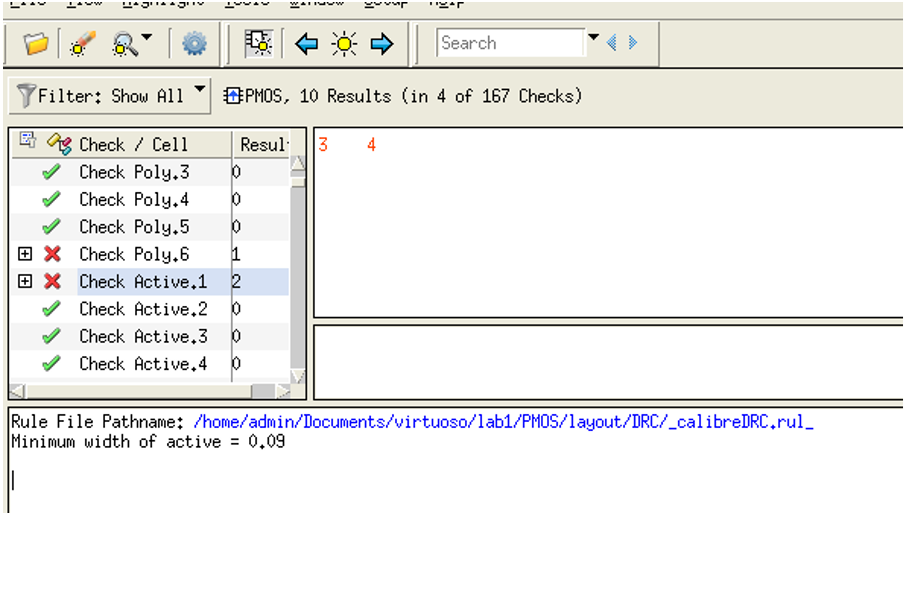
\includegraphics[width=.7\linewidth]{sections/pic/EX4_PMOS_DRC_minpoly_50.png}
	\label{f_EX4_PMOS_DRC_minpoly_50}
\end{figure}

The error occurs because the \textit{Active} region requires a minimum width of \$90n\$ but is set to \$50n\$. The small \textit{Active} region prevents the \textit{Contact} from fully covering it, resulting in the error.

\begin{figure}[H]
	\centering
	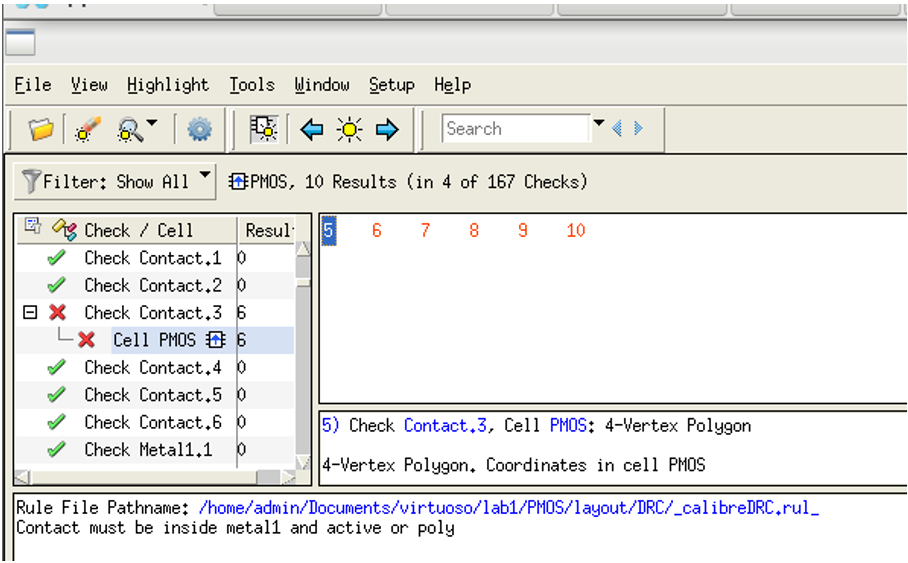
\includegraphics[width=.7\linewidth]{sections/pic/EX4_PMOS_DRC_minactive_90.png}
	\label{f_EX4_PMOS_DRC_minactive}
\end{figure}

\itemmini{Check LVS}\\

\begin{figure}[H]
	\centering
	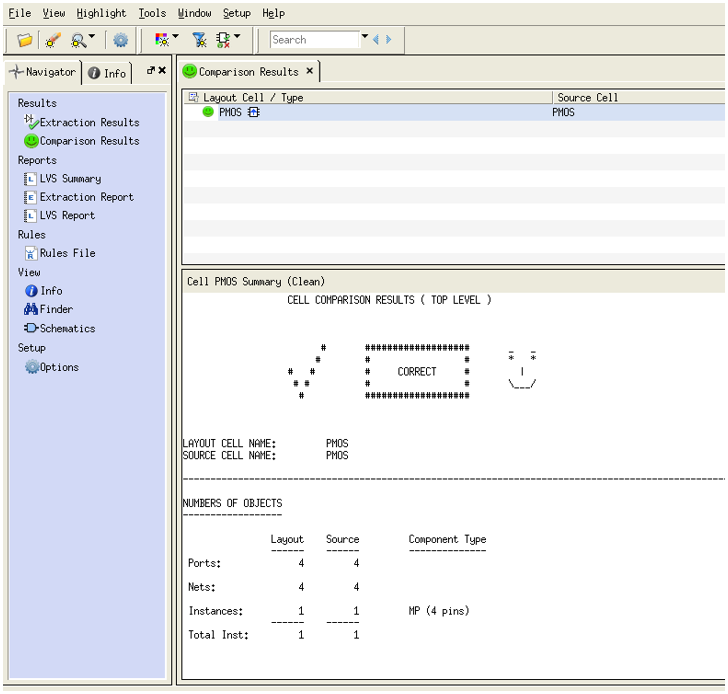
\includegraphics[width=.7\linewidth]{sections/pic/EX4_PMOS_LVS.png}
	\label{f_EX4_PMOS_LVS}
\end{figure}